\documentclass[10pt]{article}

\usepackage[margin=1in]{geometry}
\usepackage[T1]{fontenc}
\usepackage[utf8]{inputenc}
\usepackage{booktabs}
\usepackage{graphicx}
\usepackage{array}
\usepackage{tabularx}
\usepackage{longtable}
\usepackage{pdflscape}
\usepackage{adjustbox}
\usepackage{caption}
\usepackage{float}
\usepackage{hyperref}

\title{Baihu: A Billion-Frame Multi-Embodiment Robot Manipulation Dataset for Embodied Foundation Models}
\author{
Andong Chen$^{1,*}$, Renxing Feng$^{1,*}$, Yingwei Ji$^{1,*}$, Yuexuan Li$^{1,*}$, Jin Lou$^{1,*}$ \\
Xupeng Wang$^{1,*}$, Yuan Xu$^{1,*}$, Haoran Zhang$^{1,*}$, Xingdong Zhu$^{1,*}$, Yuchen Zhu$^{1,*,\dagger}$ \\
\small $^{1}$Humanoid Robotics (Shanghai) Co., Ltd. \\
\small $^{*}$All authors contributed equally to this work. \\
\small $^{\dagger}$Project lead.
}
\date{}

\begin{document}
\maketitle

\begin{figure}[H]
\centering
\includegraphics[width=\textwidth]{figures/overview.jpg}
\caption*{\textbf{Baihu overview.} Baihu contains more than 1.02 billion frames, 9521.75 hours, 513575 episodes, and 2989 tasks collected through human teleoperation across 13 physical robot platforms. Platform-specific HDF5 records are validated, aligned, and converted into LeRobot v2.1. Offline zero-shot evaluation with GR00T N1.6 uses 42 external task-dataset records excluded from Baihu training.}
\end{figure}

\begin{abstract}
Robot foundation models require paired visual, language, proprioceptive, and action supervision at a scale that exposes the physical variability of embodied interaction. Existing robot datasets remain constrained by limited embodiment coverage, heterogeneous storage conventions, weak temporal structure, and evaluation protocols that rarely test transfer outside the training corpus. \textbf{WhiteTiger} is a billion-frame, fully human-teleoperated, multi-platform robot manipulation dataset designed for foundation-model adaptation, cross-embodiment trajectory organization, and event-aware policy learning. WhiteTiger contains \textbf{9521.75 hours} of robot data, \textbf{2989 tasks}, \textbf{513575 episodes}, and \textbf{1028349814 frames} across \textbf{13 physical robot platforms}. The corpus spans fixed-base bimanual manipulators, wheeled mobile manipulators, mobile dual-arm platforms, and humanoid robots, with gripper-based and dexterous-hand end effectors. Platform-specific HDF5 operation records are converted into LeRobot v2.1 while preserving native observation, state, action, and camera schemas.

WhiteTiger couples scalable physical data collection with temporal structure. Human teleoperation grounds each trajectory in real contact dynamics, robot reachability limits, sensor placement, end-effector geometry, and embodiment-specific control spaces. Event-level annotations mark subgoal achievement, phase transitions, boundary crossings, alignment states, handover poses, deformation states, and articulated-object transitions beyond gripper or dexterous-hand actuation. Foundation-model utility is evaluated through offline open-loop zero-shot action prediction using GR00T N1.6 across \textbf{13 platforms} and \textbf{42 paired task-dataset records} from external evaluation datasets excluded from WhiteTiger training. One epoch of full fine-tuning on WhiteTiger reduces \textbf{Normalized Joint MSE by 99.42\%} and \textbf{Normalized ALL MSE by 96.79\%} relative to the no-training checkpoint. The resulting dataset supports studies of robot policy scaling, cross-embodiment adaptation, event-conditioned action generation, hierarchical skill decomposition, progress-aware value learning, and phase-aware evaluation in open-world manipulation settings.
\end{abstract}

\section{Introduction}

Scaling robot policies requires interaction data that couples perception, language, proprioception, and action under the physical constraints of embodied execution. Unlike web-scale image or text corpora, robot trajectories are bounded by robot morphology, actuator limits, camera placement, control frequency, contact dynamics, object affordances, and safety constraints. These factors determine whether policy learning captures transferable sensorimotor structure or memorizes a narrow hardware and scene distribution. Large language models and vision-language models demonstrate predictable benefits from increased data and model scale, but analogous scaling behavior in robotics depends on datasets that preserve the structure of environment-agent interaction rather than flattening embodiment-specific trajectories into weakly aligned logs~\cite{brohan2023rt1,brohan2023rt2,ghosh2024octo,kim2024openvla,black2024pi0}.

Generalist robot policies and vision-language-action models map visual observations, task descriptions, robot states, and prior context to continuous actions~\cite{driess2023palme,brohan2023rt2,kim2024openvla,black2024pi0}. Datasets such as RoboMIND~\cite{wu2024robomind}, DROID~\cite{khazatsky2024droid}, BridgeData V2~\cite{walke2023bridgedatav2}, and Open X-Embodiment~\cite{oneill2023openx} establish the value of real robot trajectories, multi-view observations, task annotations, and standardized interfaces for imitation learning. The remaining bottleneck is not only dataset size. Pretraining-oriented robot corpora must align heterogeneous embodiments, maintain physically meaningful action semantics, expose task diversity across environments and objects, and provide evaluation regimes that test transfer beyond the collected training distribution.

Dense observation-action sequences alone underrepresent the temporal structure of manipulation. Long-horizon and contact-rich tasks contain subgoals, skill boundaries, object-state changes, alignment constraints, and phase transitions that affect downstream policy learning and evaluation. Cloth folding depends on lifting peaks and folding transitions. Insertion depends on pre-insertion alignment and seated states. Container placement depends on boundary crossing. Bimanual handover depends on transfer poses and load exchange. Without explicit temporal structure, these signals must be manually engineered, heuristically recovered, or omitted, which weakens next-event prediction, event-conditioned imitation learning, hierarchical decomposition, skill-boundary detection, future-state prediction, progress-aware reward learning, and phase-aware evaluation.

\textbf{WhiteTiger} targets these constraints through a billion-frame, fully human-teleoperated, multi-platform robot manipulation corpus for embodied foundation model adaptation and event-aware learning. WhiteTiger contains \textbf{9521.75 hours} of data, \textbf{2989 tasks}, \textbf{513575 episodes}, and \textbf{1028349814 frames}. Each trajectory is collected on a physical robot platform and converted from platform-specific HDF5 source records into LeRobot v2.1~\cite{cadene2026lerobot}. The dataset therefore separates scalable training access from native control semantics: LeRobot v2.1 provides a unified loading interface, while platform-specific schemas retain the observation, proprioceptive, action, and camera conventions required for physically grounded learning.

Multi-embodiment coverage is central to the design. WhiteTiger includes fixed-base bimanual manipulators, wheeled mobile manipulators, mobile dual-arm systems, and humanoid robots. The associated control spaces range from arm-and-gripper commands to whole-body action representations involving dexterous hands, head or neck joints, waist motion, legs, and mobile bases. This heterogeneity exposes policies to variation in kinematic topology, reachable workspace, end-effector affordance, visual viewpoint, and actuation granularity. Cross-embodiment trajectory alignment is therefore treated as schema-preserving data organization rather than as an assumption that all robots share an identical action vector~\cite{bousmalis2023robocat,ghosh2024octo,xu2023xskill,liu2024rdt1b}.

Temporal structure is treated as a dataset attribute rather than an auxiliary annotation afterthought. WhiteTiger events identify frames where task progress changes measurably, including subgoal achievement, contact state transitions, object-state changes, alignment states, boundary crossings, handover poses, deformation-related states, and articulated-object transitions. These annotations extend beyond gripper or dexterous-hand opening and closing. The resulting trajectories encode both motor execution and task phase, allowing downstream methods to condition on when subgoals are reached as well as how continuous actions are produced.

The paper presents WhiteTiger through dataset construction, data standardization, and model-oriented evaluation. Dataset construction specifies human teleoperation, platform coverage, task composition, scenario distribution, skill taxonomy, robot configurations, object interactions, and event annotations. Data standardization specifies validation, quality control, metadata normalization, state-action schema alignment, and HDF5-to-LeRobot v2.1 conversion. Model-oriented evaluation uses a GR00T N1.6 checkpoint~\cite{nvidia2025grootn1} under offline open-loop zero-shot action prediction across 13 platforms and 42 paired task-dataset records from datasets external to WhiteTiger and excluded from training. One epoch of full fine-tuning on WhiteTiger reduces Normalized Joint MSE by \textbf{99.42\%} and Normalized ALL MSE by \textbf{96.79\%} relative to the no-training checkpoint.

The contribution of WhiteTiger lies in the joint combination of scale, physical human demonstration, multi-embodiment coverage, schema-preserving standardization, event-level temporal structure, and external model-oriented evaluation. The dataset provides 9521.75 hours, 2989 tasks, 513575 episodes, and 1028349814 frames across 13 physical platforms. Its HDF5-to-LeRobot v2.1 pipeline converts heterogeneous operation records into a training-ready representation while retaining platform-specific action and state semantics. Its morphology, sensing, end-effector, and control-space coverage supports cross-embodiment policy learning from gripper-based manipulation to dexterous and whole-body control. Its event annotations expose task-dependent milestones such as lifting peaks, alignment states, boundary crossings, handover poses, object-state transitions, and deformation states. Its offline zero-shot benchmark quantifies transfer from WhiteTiger fine-tuning to external evaluation datasets rather than measuring only in-corpus reconstruction.

\section{Related Work}

\subsection{Large-scale robot manipulation datasets}

Large-scale robot manipulation datasets provide the empirical substrate for generalist robot policies. Their utility depends on collection setting, embodiment coverage, task diversity, physical interaction diversity, data standardization, and evaluation design. RoboMIND provides 107k demonstration trajectories across 479 tasks and 96 object classes~\cite{wu2024robomind}. DROID collects 76k in-the-wild robot trajectories across 350 hours, 564 scenes, and 84 tasks~\cite{khazatsky2024droid}. BridgeData V2 contains 60,096 trajectories across 24 environments on a low-cost robot platform~\cite{walke2023bridgedatav2}. Open X-Embodiment aggregates data from 22 robots across 21 institutions for cross-embodiment learning at scale~\cite{oneill2023openx}.

WhiteTiger follows this data-centric direction while targeting pretraining-scale physical demonstration, cross-platform schema preservation, event-level temporal annotation, and external foundation-model evaluation. WhiteTiger contains 9521.75 hours of robot data, 2989 tasks, 513575 episodes, and 1028349814 frames. This scale places the dataset in the regime required for studying robot policy scaling under physical interaction constraints rather than only task-specific imitation learning. Recent primitive-level and intermediate-representation datasets further show that temporally structured supervision can support compositional manipulation and plan-then-execute policies~\cite{chen2024rh20tp,li2026robointer,stanovcic2026atlas}.

\begin{table}[t]
\centering
\caption{Comparison with representative large-scale robot manipulation datasets. ``Event ann.'' denotes dataset-level event or keyframe temporal milestone annotations. ``n/r'' indicates that the corresponding statistic is not reported as a primary dataset-level quantity in the cited paper. Task and skill definitions follow the conventions of each source and are therefore not directly interchangeable across datasets.}
\label{tab:dataset-comparison}
\footnotesize
\setlength{\tabcolsep}{4pt}
\renewcommand{\arraystretch}{1.08}
\begin{adjustbox}{max width=\textwidth}
\begin{tabular}{lrrrrrcl}
\toprule
Dataset & Traj. / Ep. & Hours & Platforms & Tasks & Reported skills & Event ann. & Collection \\
\midrule
BridgeData V2~\cite{walke2023bridgedatav2} & 60.1k & n/r & 1 & n/r & 13 & No & Human + scripted \\
DROID~\cite{khazatsky2024droid} & 76k & 350 & 1 & 84 & 86 & No & Human teleoperation \\
RoboMIND~\cite{wu2024robomind} & 107k & n/r & 4 & 479 & 38 & No & Human teleoperation \\
Open X-Embodiment~\cite{oneill2023openx} & $>1$M & n/r & 22 & 160266 & 527 & No & Aggregated datasets \\
\textbf{WhiteTiger} & \textbf{513.6k} & \textbf{9521.75} & \textbf{13} & \textbf{2989} & \textbf{64} & \textbf{Yes} & \textbf{Fully human teleoperation} \\
\bottomrule
\end{tabular}
\end{adjustbox}
\end{table}

Table~\ref{tab:dataset-comparison} identifies the combined position of WhiteTiger. Relative to single-platform corpora such as BridgeData V2 and DROID, WhiteTiger expands embodiment coverage and platform heterogeneity. Relative to RoboMIND, WhiteTiger contains more trajectories, tasks, and physical robot platforms. The 64-skill taxonomy reports behavioral coverage beyond task-count statistics. Open X-Embodiment covers more robot embodiments and a larger aggregate trajectory corpus through institutional aggregation. WhiteTiger instead provides a coherently managed corpus of fully human-teleoperated physical demonstrations across 13 platforms, standardized into LeRobot v2.1, with reported event-level temporal milestones and external model-oriented evaluation.

\subsection{Event-aware robot learning}

Event-aware robot learning uses sparse temporal structure to reduce effective horizon length and expose task progress. PerAct, RVT, and Act3D predict 3D keyframe or keypose actions for manipulation, while waypoint-based and hybrid-action imitation learning methods use sparse intermediate targets to anchor continuous control~\cite{shridhar2022peract,goyal2023rvt,gervet2023act3d,shi2023waypointbased,belkhale2023hydra}. Hierarchical and diffusion-based methods use sparse poses, waypoints, or skills as high-level trajectory anchors with lower-level policies generating motion between them~\cite{ke2024diffuseractor,ma2024hdp,liang2023skilldiffuser}. Skill segmentation and temporal abstraction methods decompose long-horizon demonstrations into subtasks, options, or primitive skills, making event boundaries natural supervision for hierarchical policies and diagnostic evaluation~\cite{shiarlis2018taco,pertsch2020spirl,mao2024dexskills}.

Intermediate-representation methods expose additional structure between task instructions and low-level actions. Vision-language-action systems introduce language motions, embodied reasoning traces, future visual states, contact phases, or per-frame intermediate labels~\cite{belkhale2024rth,zawalski2024ecot,zhao2025cotvla,li2025switchvla,li2026robointer}. Video-planning and generative robot models use visual subgoals or future frames as planning targets~\cite{du2023unipi,wu2023gr1,zhao2025cotvla}. Reward and value learning methods use visual or language-aligned progress signals to shape policy learning~\cite{zakka2021xirl,ma2022vip,ma2023liv,sontakke2023roboclip}. WhiteTiger supplies event annotations as general temporal structure supervision for next-event prediction, event-to-event action generation, hierarchical policy learning, skill-boundary detection, VLA intermediate supervision, future-state prediction, progress-aware reward learning, and phase-aware evaluation.

\subsection{Multi-embodiment robot learning}

Multi-embodiment learning trains policies that benefit from trajectories collected on heterogeneous robot platforms. The central difficulty is not platform count alone. Robot datasets differ in kinematic topology, joint dimensionality, end-effector design, gripper conventions, dexterous-hand actuation, camera placement, control frequency, coordinate frames, and task distribution. Prior work has studied multi-robot datasets, cross-embodiment policy learning, and adaptation to unseen robot configurations~\cite{dasari2020robonet,oneill2023openx,bousmalis2023robocat,ghosh2024octo,xu2023xskill,liu2024rdt1b}.

WhiteTiger provides multi-embodiment trajectories across fixed-base manipulation, wheeled mobile manipulation, mobile dual-arm operation, and humanoid whole-body control. Its platforms use different sensing arrangements, parallel grippers, dexterous hands, and heterogeneous action-state schemas. The dataset is therefore suited to studying schema-preserving robot data standardization, cross-platform policy training, and action prediction under embodiment-dependent physical constraints.

\subsection{Vision-language-action models}

Vision-language-action models learn sensorimotor mappings from visual observations, language instructions, robot state, and context to robot actions. Recent embodied models combine multimodal foundation models with continuous robot control representations to support generalist policies~\cite{driess2023palme,brohan2023rt2,ghosh2024octo,kim2024openvla,black2024pi0,nvidia2025grootn1}. Their generalization depends on synchronized observation-action trajectories, reliable task-level annotations, physically meaningful action labels, and sufficient variation across environments, objects, and embodiments.

WhiteTiger supports this paradigm by organizing human-teleoperated robot trajectories as standardized observation-action sequences in LeRobot v2.1~\cite{cadene2026lerobot}. The benchmark evaluates this data foundation through offline open-loop zero-shot action prediction using GR00T N1.6 checkpoints~\cite{nvidia2025grootn1} on datasets external to WhiteTiger.

\subsection{Data standardization for robot learning}

Robot data standardization is a prerequisite for large-scale policy learning across heterogeneous platforms. Raw operation logs often differ in state definitions, action dimensions, camera streams, gripper conventions, control rates, timestamp conventions, and metadata schemas. A unified policy cannot be trained reliably when state-action dimensions are misaligned, camera streams are ambiguously named, or task labels are inconsistent~\cite{dasari2020robonet,oneill2023openx,ghosh2024octo}.

WhiteTiger addresses this problem through structured dataset management and HDF5-to-LeRobot v2.1 conversion. The management layer tracks data additions, cleaning, normalization changes, and embodiment-specific schema fixes. The LeRobot v2.1 representation provides a training-oriented interface for scalable loading, sharing, and evaluation. This design is critical in pretraining-scale robot corpora because small state-action mapping errors can propagate across many training runs and distort measured scaling behavior.

\subsection{Positioning of WhiteTiger}

WhiteTiger is positioned as a billion-frame, fully human-teleoperated, multi-platform robot manipulation dataset for embodied foundation model adaptation and event-aware robot learning. Its defining property is the joint presence of physical demonstration scale, multi-embodiment morphology, platform-specific schema preservation, HDF5-to-LeRobot v2.1 standardization, event-level temporal annotation, and external offline evaluation with a foundation-model checkpoint. The dataset complements single-hardware corpora and aggregated multi-institution datasets by providing a coherently organized, temporally structured, and model-oriented data foundation for open-world manipulation policy learning.

\section{WhiteTiger Dataset}

\subsection{Dataset scale}

WhiteTiger contains \textbf{9521.75 hours} of robot manipulation data, \textbf{2989 tasks}, \textbf{513575 episodes}, and \textbf{1028349814 frames} across \textbf{13 robot platforms}. The corpus targets foundation-model adaptation and policy scaling rather than isolated task-specific imitation.

The total frame count and duration imply an average recording rate of approximately 30 frames per second. The average episode contains approximately 2002 frames, corresponding to approximately 66.7 seconds. These quantities define the temporal density available for learning continuous sensorimotor mappings and the episode-level horizon distribution that constrains open-loop and closed-loop policy evaluation.

\subsection{Skill taxonomy}

Baihu covers 64 manipulation skills across 2989 tasks. Rather than treating tasks as isolated labels, the dataset organizes manipulation behaviors through a reusable set of skill-level action semantics. These skills describe both low-level motion primitives and higher-level manipulation interactions, including object acquisition, placement, handover, articulated object interaction, contact-based motion, tool and material manipulation, and navigation-related actions.

Table~\ref{tab:skill-taxonomy} summarizes the 64 skills according to seven action-semantic categories. This taxonomy provides an intermediate level between individual task names and raw action trajectories: a single task may involve multiple skills, and the same skill can appear across different objects, scenes, and robot embodiments. This structure helps characterize the manipulation diversity of Baihu beyond simple task count.

% Baihu v2.0 skill taxonomy table generated from materials/技能.csv.
% Required packages: booktabs, tabularx, adjustbox.

\begin{table}[t]
\centering
\caption{Skill taxonomy of Baihu v2.0. The 64 manipulation skills are grouped according to their action semantics during data collection and annotation.}
\label{tab:skill-taxonomy}
\footnotesize
\setlength{\tabcolsep}{4pt}
\renewcommand{\arraystretch}{1.15}
\begin{adjustbox}{max width=\textwidth}
\begin{tabularx}{\textwidth}{p{0.30\textwidth}p{0.08\textwidth}X}
\toprule
Category & Count & Skills \\
\midrule
Object acquisition and release & 9 & Grasp, Pick, Pick up, Pinch, Suction, Hold, Lift, Lower, Release \\
Transport, placement, and handover & 10 & Move, Place, Carry, Transfer, HandOver, TakeOver, Throw, Discard, Takeout, Remove \\
Spatial arrangement and organization & 8 & Alignment, Adjust, Straighten, Stack, Unstack, Pack, Ensure, Several Times \\
Articulated, container, and electrical interaction & 11 & Open, Close, OpenBox, CloseBox, DrawOut, Insert, Plug, Unplug, PressButton, Zip, Unzip \\
Contact-based motion primitives & 9 & Push, Pull, Press, Rotate, Flip, Stretch, Touch, Swipe, Shake \\
Tool, fluid, and material manipulation & 10 & Pour, Scoop, Wipe, Water, Brush, Stir, Stick, Tear, Fold, Unfold \\
Navigation, perception, and expressive actions & 7 & Navigate, Point, Scan, Check, Hang, Armretract, Wave \\
\midrule
\textbf{Total} & \textbf{64} & -- \\
\bottomrule
\end{tabularx}
\end{adjustbox}
\end{table}


\subsection{Robot platform composition}

Baihu contains data from 13 robot platforms, covering a diverse set of robot embodiments and data sources. Table~\ref{tab:platform-comp} summarizes the platform-level composition of the dataset in terms of task count, episode count, frame count, and total duration. This platform-level reporting provides transparency about the dataset source composition while keeping the main emphasis on overall scale, platform coverage, and standardized data organization.

\begin{table}[t]
\centering
\caption{Platform-level composition of Baihu. The table reports tasks, episodes, frames, and hours for each of the 13 robot platforms.}
\label{tab:platform-comp}
\scriptsize
\begin{tabular}{lrrrr}
\toprule
Robot platform & Tasks & Episodes & Frames & Hours \\
\midrule
ARX\_Loong & 3 & 842 & 2223107 & 20.58 \\
Astribot S1 & 100 & 29889 & 40932735 & 379.01 \\
Agilex Cobot Magic & 112 & 33098 & 55115692 & 510.33 \\
UR5e & 49 & 14805 & 22939047 & 212.40 \\
D-Wheel & 231 & 13485 & 36172626 & 334.93 \\
Franka & 9 & 2090 & 4037181 & 37.38 \\
Agibot GO-1 & 1512 & 140718 & 459379181 & 4253.51 \\
Fourier GR-2 & 319 & 96686 & 103615634 & 959.40 \\
Leju KUAVO & 123 & 29095 & 42586155 & 394.32 \\
QingLong & 167 & 46506 & 91909479 & 851.01 \\
Tianji & 6 & 1575 & 2727875 & 25.26 \\
Galaxea R1 & 239 & 70111 & 96863491 & 896.88 \\
Agibot A2 & 119 & 34675 & 69847611 & 646.74 \\
\textbf{Total} & \textbf{2989} & \textbf{513575} & \textbf{1028349814} & \textbf{9521.75} \\
\bottomrule
\end{tabular}
\end{table}

The platform composition in Table~\ref{tab:platform-comp} shows that Baihu integrates robot operation data from multiple platforms with different embodiments, control interfaces, and task settings. This coverage supports unified data standardization and cross-platform model evaluation while preserving platform-specific state and action schemas.

\subsection{Scenario and task coverage}

Beyond scale and embodiment diversity, Baihu is designed to cover a broad range of manipulation scenarios and task structures. The dataset is intended to support robot learning in both daily-life and production-oriented environments. Representative scenario families include industrial manufacturing, household service, catering or food handling, retail or pharmacy-like environments, and other generalization scenarios. These scenario categories provide a practical organization for analyzing how robot policies transfer across environments and object distributions.

At the task level, Baihu contains 2989 tasks. These tasks include both short-horizon primitive behaviors and longer-horizon task chains. Many tasks can be viewed as compositions of lower-level manipulation skills, such as grasping, placing, pushing, pulling, handing over, inserting, pressing, opening, closing, sorting, and arranging. This composition makes the dataset useful not only for direct action prediction, but also for studying how low-level manipulation skills combine into longer task sequences.

\subsection{Object and interaction diversity}

Baihu contains robot interactions with diverse real-world objects. The objects span household items, kitchen utensils, retail goods, packages, industrial parts, tools, flexible materials, and irregularly shaped objects. These objects differ in size, shape, material, rigidity, surface texture, and manipulation affordance. Such object diversity is important for learning policies that do not overfit to a small set of familiar objects.

The dataset also includes different interaction patterns between robots and objects. Some trajectories involve single-object pick-and-place behaviors, while others involve object sorting, tool use, assembly-like manipulation, container interaction, drawer or door operation, and multi-object organization. This diversity supports the study of generalization across objects, tasks, and physical interaction types.

\subsection{Temporal horizon and skill composition}

Robot manipulation tasks in Baihu span multiple temporal horizons. Short-horizon trajectories typically correspond to local operations such as grasping, pressing, scanning, or simple placement. Medium-horizon trajectories may include object transfer, opening and closing, sorting, or simple multi-step rearrangement. Long-horizon trajectories involve more extended task chains, such as cleaning, assembly, loading or unloading, and multi-stage object organization.

This temporal diversity is important for embodied foundation model training. Short trajectories provide dense examples of low-level visuomotor control, while longer trajectories expose models to task phases, intermediate goals, action rhythm, and sequential dependencies. As a result, Baihu can support both low-level action prediction and higher-level behavior modeling.

\subsection{Data format}

Baihu is converted from HDF5 source records into the LeRobot v2.1 format. Each episode is represented as a trajectory consisting of temporally ordered observation-action pairs. Depending on the original robot platform and task setup, each trajectory may include visual observations, robot state information, action commands, task labels, and metadata. The standardized format is intended to support direct loading by robot learning pipelines and large-scale model training systems.

A typical Baihu trajectory can be represented as a task instruction or task label, synchronized visual observations, robot proprioceptive states, robot actions, episode metadata, and frame-level timestamps or ordering information.

\section{Data Processing Pipeline}

Baihu converts heterogeneous human-teleoperated robot operation records into a consistent dataset for large-scale policy training. The source trajectories are stored in HDF5 format and are standardized into LeRobot v2.1 for downstream imitation-learning and vision-language-action training. The processing pipeline emphasizes three requirements: preserving embodiment-specific control information, filtering invalid or task-inconsistent trajectories, and producing a unified representation that can be loaded by modern robot learning systems.

\subsection{HDF5 ingestion and trajectory validation}

Raw Baihu trajectories are first organized as HDF5 records. Each record is associated with a robot platform, task identity, episode identity, and available modality fields. Depending on the source platform and task setup, a trajectory may include visual observations, robot proprioceptive states, robot actions, task annotations, timestamps, and episode-level metadata.

Because Baihu integrates data from multiple robot platforms, validation is required before data enters the released training corpus. The pipeline checks whether each episode contains temporally ordered observations and actions, usable modality fields, consistent task metadata, valid platform information, and aligned observation-action sequences. This validation step removes incomplete, corrupted, or unusable trajectories that would otherwise provide incorrect supervision during model training.

\subsection{Quality control and metadata standardization}

Baihu uses a multi-stage quality control workflow covering data acquisition, monitoring, upload, validation, cleaning, review, and final delivery. This workflow is important at the scale of Baihu because even a small fraction of invalid trajectories can correspond to a large amount of unusable data. Quality control therefore aims to maintain consistency across heterogeneous platforms while preserving the diversity needed for embodied model pretraining.

A trajectory is retained only when it satisfies the task request under which it was collected. Trajectories that do not follow the task requester specification are removed from the dataset. Typical removal cases include incorrect scene setup, incorrect objects or tools, wrong manipulation procedure, incomplete task execution, corrupted recordings, missing modality fields, inconsistent task metadata, or misaligned observation-action sequences. As a result, Baihu does not intentionally preserve failed or task-inconsistent demonstrations as training examples in the released corpus.

Task and episode metadata are standardized to support dataset analysis and model conditioning. Each episode is associated with task information, platform metadata, and source-specific fields when available. These annotations enable analysis by task and platform, and they also provide the language or semantic conditioning signals used by vision-language-action policies. Since task annotations are manually provided when collection requirements are proposed, metadata standardization also checks that the recorded trajectory remains consistent with the intended task description.

\subsection{State and action schema alignment}

State and action representations differ across robot platforms. Platforms may have different joint layouts, gripper or hand structures, control frequencies, and action semantics. Baihu therefore preserves platform-specific schemas that define which dimensions correspond to arm joints, grippers, hands, or other controllable components.

This schema alignment is important for both training and evaluation. It allows each platform to retain its native control representation while enabling unified dataset loading. It also supports metric definitions such as Joint MSE and ALL MSE: Joint MSE uses only joint-related action dimensions, while ALL MSE uses the full action vector for each platform.

For grippers and hands, values are stored according to the actual physical travel range of each platform. Baihu does not impose a single universal gripper or hand scale across robots. This design keeps the stored action values faithful to the original robot control space and avoids forcing heterogeneous end-effectors into an artificial shared range.

\subsection{HDF5-to-LeRobot v2.1 conversion}

After validation and schema alignment, Baihu is converted from the source HDF5 records into the LeRobot v2.1 format. The conversion standardizes episode and frame organization, synchronized visual observations, robot states, actions, human-provided task annotations, and episode-level metadata. This separates the source storage format from the model-training representation: HDF5 provides the original trajectory container, while LeRobot v2.1 provides a consistent interface for dataset loading, episode management, and downstream training.

Because the robot platforms have different embodiments and control spaces, Baihu does not force all platforms into an identical observation or action vector. Instead, each platform retains its modality-specific state, action, and camera schema within the shared LeRobot v2.1 interface. This design enables consistent data access across platforms while preserving the physical control semantics of each robot.

\section{Benchmark Experiments}

To demonstrate the value of Baihu for embodied foundation model training, we evaluate whether a model trained on Baihu improves offline action prediction on external evaluation datasets. The datasets used for open-loop evaluation are not part of the Baihu training corpus. The benchmark therefore measures transfer from Baihu pretraining to held-out evaluation trajectories collected separately from Baihu.

\subsection{Offline open-loop zero-shot evaluation}

Open-loop evaluation provides an offline assessment by comparing the model's predicted actions against reference actions from human-teleoperated robot demonstrations. In this benchmark, we compare a no-training GR00T N1.6 checkpoint~\cite{nvidia2025grootn1}, checkpoint-1, with checkpoint-390000, which was trained on Baihu for one epoch. The evaluation covers \textbf{13 platforms} and \textbf{42 paired task-dataset records} drawn from datasets that are external to Baihu and excluded from Baihu training. No additional finetuning is performed on these evaluation datasets. We therefore use zero-shot to denote dataset-level transfer from Baihu pretraining to external held-out evaluation data.

\subsection{Evaluation protocol}

For each task-dataset record, five trajectories are randomly sampled from the corresponding external evaluation dataset. The same sampled trajectories are then used to evaluate both checkpoints, providing a paired comparison between the no-training baseline and the Baihu-trained model. The model predicts actions from the recorded observations of each trajectory, and the prediction error is measured against the associated human-teleoperation actions. Predictions are generated with an action horizon of 30, and each trajectory is evaluated over its available length up to a maximum of 3000 steps. The task-level result is obtained by averaging the trajectory-level MSE values over the five trajectories.

Per-platform results are computed as the unweighted mean over the task-dataset records associated with each platform. The overall benchmark result is then reported as the unweighted mean across all 42 paired task-dataset records. This evaluation design gives each task-dataset record equal weight, independent of the amount of data available for a particular platform or task.

\subsection{Evaluation metrics}

All reported MSE values are normalized by action range to make errors more comparable across platforms with different action scales. For a trajectory with $T$ evaluated timesteps and a selected set of $D$ action dimensions, the normalized MSE is defined as

\begin{equation}
\mathrm{NMSE}
=
\frac{1}{TD}
\sum_{t=1}^{T}
\sum_{d=1}^{D}
\left(
\frac{\hat{a}_{t,d}-a_{t,d}}
{a_{d}^{\max}-a_{d}^{\min}}
\right)^{2},
\label{eq:normalized-mse}
\end{equation}

where $a_{t,d}$ and $\hat{a}_{t,d}$ denote the reference and predicted action values for dimension $d$ at timestep $t$, respectively, and $a_{d}^{\max}-a_{d}^{\min}$ is the corresponding action range. The same action normalization statistics are used for checkpoint-1 and checkpoint-390000, ensuring that the two checkpoints are compared under an identical metric scale.

\textbf{Normalized ALL MSE} is used as the primary evaluation metric. In Eq.~\ref{eq:normalized-mse}, $D$ includes the complete action vector, consisting of robot joint actions and end-effector actuation dimensions such as grippers or dexterous hands.

\textbf{Normalized Joint MSE} is reported as an auxiliary diagnostic metric. In this case, $D$ includes only robot joint action dimensions and excludes end-effector actuation dimensions, which may correspond to a gripper or a dexterous hand depending on the platform. This separation enables joint-motion prediction to be analyzed independently from platform-specific end-effector control.

\subsection{Overall results}

The benchmark results show that one epoch of training on Baihu substantially reduces normalized offline open-loop prediction error across the 13 evaluated platforms and 42 external paired task-dataset records. At the aggregate level, the Baihu-trained checkpoint reduces Normalized ALL MSE from 0.157283 to 0.005051, corresponding to a \textbf{96.79\%} relative improvement. It also reduces Normalized Joint MSE from 0.116746 to 0.000680, corresponding to a \textbf{99.42\%} relative improvement. The per-platform comparisons are visualized in Fig.~\ref{fig:per-platform-zero-shot}.

This indicates that Baihu provides effective supervision for improving full-vector and joint-related action prediction on evaluation data that were not included in the Baihu training corpus.

\subsection{Per-platform results}

Because Baihu is a multi-embodiment dataset, aggregate metrics alone are insufficient. We therefore also analyze the results separately for each evaluated platform. Across all 13 platforms, the Baihu-trained checkpoint achieves lower Normalized ALL MSE and Normalized Joint MSE than the no-training baseline.

\begin{figure}[t]
\centering
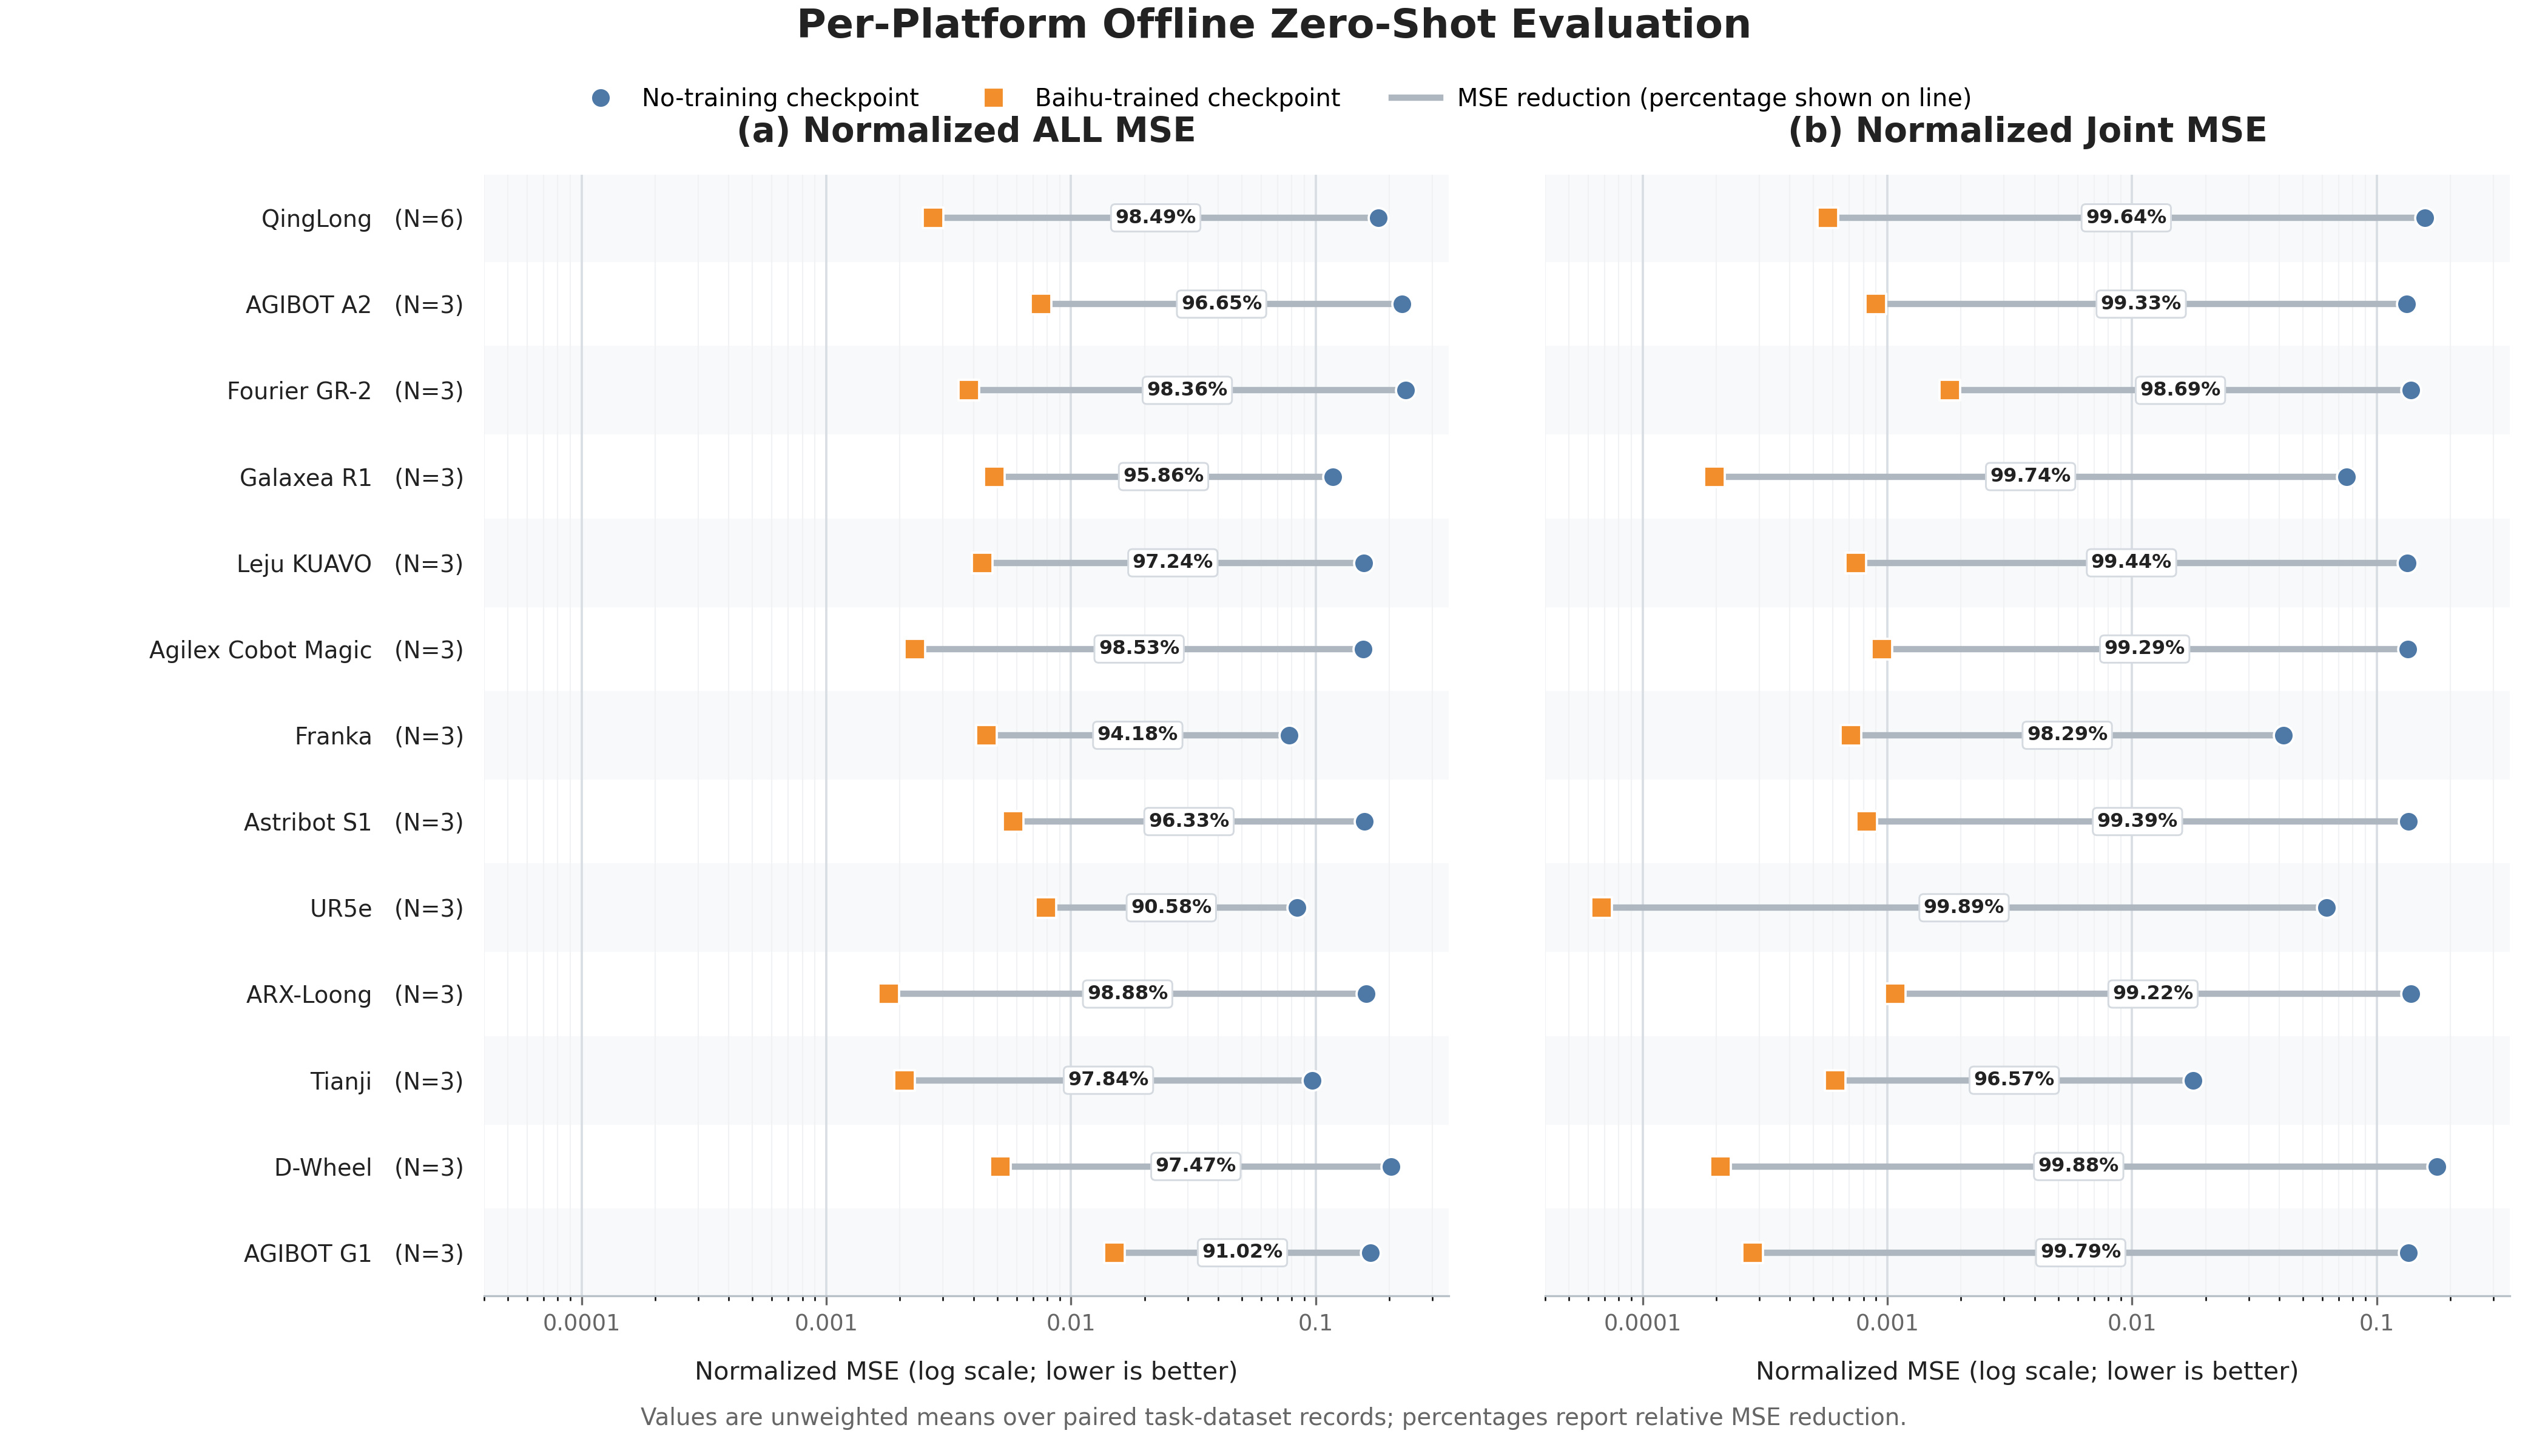
\includegraphics[width=\textwidth]{figures/per_platform_zero_shot_dumbbell.jpg}
\caption{Per-platform offline zero-shot evaluation on datasets external to Baihu. Each row compares the no-training GR00T N1.6 checkpoint (checkpoint-1) with the checkpoint trained on Baihu for one epoch (checkpoint-390000) for Normalized ALL MSE and Normalized Joint MSE. Connected markers show the change after Baihu training; lower is better. Each platform value is the unweighted mean over its paired task-dataset records. QingLong contains six records, while each of the remaining platforms contains three.}
\label{fig:per-platform-zero-shot}
\end{figure}

Figure~\ref{fig:per-platform-zero-shot} shows that the improvement is consistent rather than being driven by a small subset of embodiments. Relative reductions range from 90.58\% to 98.88\% for Normalized ALL MSE and from 96.57\% to 99.89\% for Normalized Joint MSE. Joint prediction improves particularly uniformly across platforms, whereas the remaining ALL MSE varies more because it additionally includes platform-specific end-effector dimensions such as grippers and dexterous hands. These results support the use of Baihu as a shared pretraining corpus for heterogeneous robot embodiments.

\subsection{Task-level analysis}

Task-level results further show that Baihu training improves normalized offline prediction across the 42 external paired task-dataset records. Task-level reporting is especially useful because different platforms may have different action spaces, control frequencies, and end-effector structures.

Table~\ref{tab:task-level} reports Normalized ALL MSE, Normalized Joint MSE, and relative improvement for each of the 42 paired task-dataset records. The full task-level table is provided in Appendix~\ref{app:task-level}.

The strongest improvements are observed on records where the no-training checkpoint has relatively large action prediction error. The remaining residual errors after Baihu training are small in absolute value, but they can still vary across platforms and tasks due to differences in action representation and task dynamics.

\subsection{Additional benchmark extensions}

The current benchmark provides a dataset-level held-out offline zero-shot comparison. Future versions can extend the benchmark with data-scaling evaluation, held-out platform evaluation, closed-loop simulation evaluation, and real-world rollout success rate.

\section{Discussion and Limitations}

Baihu provides a large-scale and standardized data foundation for embodied intelligence research. Its main strengths lie in its scale, fully human-teleoperated collection protocol, multi-platform coverage, preservation of platform-specific observation and action schemas, and conversion into the LeRobot v2.1 format. With \textbf{9521.75 hours}, \textbf{513575 episodes}, and more than \textbf{1.03 billion frames} of robot data, Baihu supports pretraining regimes that are difficult to study using smaller task-specific datasets.

The offline zero-shot benchmark provides initial evidence that Baihu is useful for embodied foundation model pretraining. The evaluation datasets are external to Baihu and are excluded from Baihu training. Across 13 platforms and 42 paired task-dataset records, the Baihu-trained GR00T N1.6 checkpoint substantially reduces both Normalized ALL MSE and Normalized Joint MSE compared with the no-training checkpoint. Each task-level result is averaged over five evaluation trajectories, and both checkpoints are evaluated on the same trajectories. These results suggest that Baihu pretraining transfers effectively to separately collected robot demonstration data.

At the same time, the current benchmark should be interpreted as an offline action-prediction evaluation rather than a complete measure of real-world robot performance. Open-loop normalized MSE measures agreement with reference teleoperation actions, but it does not capture closed-loop recovery, compounding errors, contact-rich interaction, or task success under real robot execution. Moreover, the benchmark demonstrates dataset-level transfer because the evaluation datasets are external to Baihu, but it should not be interpreted as a held-out-platform experiment when the evaluated robot platform is also represented in Baihu.

Another limitation is that the current paper focuses on a single primary benchmark setting: a GR00T N1.6 checkpoint comparison under offline open-loop evaluation. Additional baselines such as ACT, Diffusion Policy, or other vision-language-action policies would make the benchmark more comprehensive. Data-scaling experiments, held-out-platform evaluation, and closed-loop robot rollouts would further clarify which aspects of Baihu contribute most to model performance. The current benchmark also uses an unweighted mean across task-dataset records; future work could additionally report trajectory-weighted results and uncertainty estimates across evaluation trajectories.
\section{Conclusion}

We introduced \textbf{Whitetiger}, a billion-frame, fully human-teleoperated, multi-platform robot manipulation dataset for embodied foundation model adaptation and event-aware robot learning. Whitetiger contains \textbf{9521.75 hours} of robot data, \textbf{2989 tasks}, \textbf{513575 episodes}, and \textbf{1028349814 frames} across \textbf{13 robot platforms}. The dataset converts platform-specific HDF5 robot operation records into the LeRobot v2.1 format, providing a standardized data foundation for training vision-language-action models and generalist robot policies.

Whitetiger combines two complementary dataset properties: scale and temporal structure. Its large-scale dense trajectories support foundation-model adaptation and offline zero-shot action prediction on datasets external to Whitetiger. Its event- and keyframe-level temporal annotations expose task progress and semantic milestones beyond gripper or dexterous-hand state changes. These annotations make Whitetiger compatible with keyframe-aware learning paradigms such as waypoint-conditioned imitation learning, goal-conditioned policy learning, hierarchical skill decomposition, reward shaping, value-guided policy improvement, subgoal-image reasoning, and phase-aware evaluation.

We evaluated the utility of Whitetiger through offline open-loop zero-shot evaluation on external datasets excluded from Whitetiger training. Across 13 platforms and 42 paired task-dataset records, a GR00T N1.6 model trained on Whitetiger for one epoch reduced \textbf{Normalized ALL MSE by 96.79\%} and \textbf{Normalized Joint MSE by 99.42\%} compared with the no-training baseline. Each task-level result was averaged over five evaluation trajectories. These results suggest that Whitetiger provides effective large-scale supervision for robot action prediction and can serve as practical infrastructure for future embodied foundation model development.

Future work will extend Whitetiger with additional benchmark protocols, more baseline models, closed-loop evaluations, data-scaling studies, held-out-platform evaluation, and clearer release documentation. A planned real-world comparison between dense trajectory training and event-derived value supervision will evaluate whether Whitetiger temporal annotations improve real-robot execution success rate. Together, these directions can further strengthen Whitetiger as a reusable data foundation for large-scale and temporally structured embodied intelligence research.


\appendix
\section{Task-level benchmark results}
\label{app:task-level}

% A4-width replacement for Appendix Table 7 / task-level benchmark table.
% Use inside main.tex after \section{Task-level benchmark results}.
% Required packages: booktabs, longtable, array, pdflscape.

\begingroup
\begin{landscape}
\tiny
\setlength{\tabcolsep}{2pt}
\renewcommand{\arraystretch}{1.05}
\setlength{\LTleft}{0pt}
\setlength{\LTright}{0pt}

\begin{longtable}{@{}p{0.085\linewidth}p{0.300\linewidth}p{0.070\linewidth}rrrrrr@{}}
\caption{Task-level offline zero-shot evaluation results. The table reports Joint MSE, ALL MSE, and relative improvement for each of the 42 paired task-dataset records. Lower MSE is better.}\label{tab:task-level}\\
\toprule
Platform & Task & Type & Joint-1 & Joint-Baihu & $\Delta$Joint & ALL-1 & ALL-Baihu & $\Delta$ALL \\
\midrule
\endfirsthead
\caption[]{Task-level offline zero-shot evaluation results (continued).}\\
\toprule
Platform & Task & Type & Joint-1 & Joint-Baihu & $\Delta$Joint & ALL-1 & ALL-Baihu & $\Delta$ALL \\
\midrule
\endhead
\midrule
\multicolumn{9}{r}{Continued on next page}\\
\endfoot
\bottomrule
\endlastfoot
Qinglong & Put a ballpoint pen into a pen holder &  & 0.179469 & 0.000248 & 99.86\% & 0.201477 & 0.003823 & 98.10\% \\
Qinglong & Sort fruits and vegetables into baskets &  & 0.183410 & 0.000527 & 99.71\% & 0.207567 & 0.005064 & 97.56\% \\
Qinglong & Throw trash into a trash can & Dual-arm & 0.132497 & 0.000339 & 99.74\% & 0.160485 & 0.000669 & 99.58\% \\
Qinglong & Cover a pot with a lid &  & 0.180345 & 0.000200 & 99.89\% & 0.202733 & 0.002103 & 98.96\% \\
Qinglong & Place an egg & Dual-arm & 0.133400 & 0.001388 & 98.96\% & 0.162696 & 0.001901 & 98.83\% \\
Qinglong & Pack food & Dual-arm & 0.133672 & 0.000732 & 99.45\% & 0.148295 & 0.002839 & 98.09\% \\
Zhiyuan A2 & Sort eggplants and bananas with a yellow-grid tabletop background & Dual-arm & 0.132409 & 0.000713 & 99.46\% & 0.222947 & 0.006068 & 97.28\% \\
Zhiyuan A2 & Sort black and white tape with a small-fish-towel tabletop background & Dual-arm & 0.133624 & 0.001356 & 98.99\% & 0.227667 & 0.011405 & 94.99\% \\
Zhiyuan A2 & Sort cross-shaped and cylindrical blocks with a red tabletop background & Dual-arm & 0.132239 & 0.000620 & 99.53\% & 0.225768 & 0.005214 & 97.69\% \\
Fourier GR-2 & Place a toy duck & Dual-arm & 0.137008 & 0.001172 & 99.14\% & 0.244131 & 0.003854 & 98.42\% \\
Fourier GR-2 & Sort toys & Dual-arm & 0.139023 & 0.001794 & 98.71\% & 0.231410 & 0.003836 & 98.34\% \\
Fourier GR-2 & Sort green and yellow pears & Dual-arm & 0.137948 & 0.002447 & 98.23\% & 0.226048 & 0.003783 & 98.33\% \\
Xinghaitu R1 & Put a spoon into a plate & Right-arm & 0.068287 & 0.000107 & 99.84\% & 0.110777 & 0.005057 & 95.44\% \\
Xinghaitu R1 & Sort apples and pears & Dual-arm & 0.082550 & 0.000211 & 99.74\% & 0.124586 & 0.003934 & 96.84\% \\
Xinghaitu R1 & Put a T-shirt into a basket & Right-arm & 0.075271 & 0.000274 & 99.64\% & 0.117380 & 0.005601 & 95.23\% \\
Leju KUAVO & Place a kettle & Left-arm & 0.133692 & 0.000806 & 99.40\% & 0.158527 & 0.004078 & 97.43\% \\
Leju KUAVO & Place an egg & Right-arm & 0.133315 & 0.000456 & 99.66\% & 0.155686 & 0.004150 & 97.33\% \\
Leju KUAVO & Open a drawer, place an object inside, and close it & Dual-arm & 0.133361 & 0.000969 & 99.27\% & 0.157571 & 0.004777 & 96.97\% \\
Songling Aloha & Put vegetable blocks into a bowl and center the container &  & 0.133895 & 0.000616 & 99.54\% & 0.159897 & 0.001871 & 98.83\% \\
Songling Aloha & Pick and place chopsticks in a drawer and align tableware &  & 0.134391 & 0.001479 & 98.90\% & 0.151264 & 0.002772 & 98.17\% \\
Songling Aloha & Put strawberries on a plate and stack cups &  & 0.133619 & 0.000752 & 99.44\% & 0.158443 & 0.002277 & 98.56\% \\
Franka FR3 & Stack cups & Dual-arm & 0.051757 & 0.000510 & 99.02\% & 0.086843 & 0.002837 & 96.73\% \\
Franka FR3 & Organize objects & Dual-arm & 0.038663 & 0.000731 & 98.11\% & 0.074911 & 0.005935 & 92.08\% \\
Franka FR3 & Place a toy duck & Dual-arm & 0.034437 & 0.000892 & 97.41\% & 0.071658 & 0.004803 & 93.30\% \\
Astribot S1 & Put a bowl onto a plate with a green tabletop background & Right-arm & 0.134600 & 0.000700 & 99.48\% & 0.159800 & 0.003900 & 97.56\% \\
Astribot S1 & Put a spoon into a bowl with a green-grid tabletop background & Right-arm & 0.135232 & 0.000892 & 99.34\% & 0.155694 & 0.007153 & 95.41\% \\
Astribot S1 & Place a cup and saucer with an orange tabletop background & Right-arm & 0.135401 & 0.000875 & 99.35\% & 0.160526 & 0.006405 & 96.01\% \\
UR5e & Put a coin into a piggy bank & Right-arm & 0.062034 & 0.000031 & 99.95\% & 0.085492 & 0.010285 & 87.97\% \\
UR5e & Stack blocks & Dual-arm & 0.062204 & 0.000131 & 99.79\% & 0.081088 & 0.008773 & 89.18\% \\
UR5e & Semantic test & Dual-arm & 0.062930 & 0.000041 & 99.94\% & 0.084983 & 0.004632 & 94.55\% \\
ARX & Fold clothes & Dual-arm & 0.137219 & 0.000791 & 99.42\% & 0.156832 & 0.001914 & 98.78\% \\
ARX & Fold clothes with revised procedure & Dual-arm & 0.140643 & 0.002073 & 98.53\% & 0.166439 & 0.002632 & 98.42\% \\
ARX & Fold clothes with detailed handling & Dual-arm & 0.136654 & 0.000363 & 99.73\% & 0.160718 & 0.000862 & 99.46\% \\
Tianji & Arrange flowers & Dual-arm & 0.017314 & 0.000778 & 95.50\% & 0.089298 & 0.002285 & 97.44\% \\
Tianji & Sort batteries & Dual-arm & 0.016675 & 0.000329 & 98.03\% & 0.106140 & 0.001487 & 98.60\% \\
Tianji & Stack cups & Dual-arm & 0.019495 & 0.000730 & 96.26\% & 0.095306 & 0.002505 & 97.37\% \\
Dwheel & Sort octopus toys with a small-fish-towel tabletop background & Dual-arm & 0.176082 & 0.000165 & 99.91\% & 0.203914 & 0.005410 & 97.35\% \\
Dwheel & Sort green and yellow pears with a blue-grid tabletop background & Dual-arm & 0.176593 & 0.000242 & 99.86\% & 0.203826 & 0.006220 & 96.95\% \\
Dwheel & Sort cylindrical and cuboid blocks with a green-grid tabletop background & Dual-arm & 0.176471 & 0.000217 & 99.88\% & 0.203759 & 0.003841 & 98.11\% \\
Zhiyuan G1 & Install a bracket & Right-arm & 0.135378 & 0.000409 & 99.70\% & 0.167892 & 0.013138 & 92.17\% \\
Zhiyuan G1 & Install a power module & Dual-arm & 0.135268 & 0.000291 & 99.78\% & 0.165634 & 0.012706 & 92.33\% \\
Zhiyuan G1 & Assemble a touchpad & Dual-arm & 0.134856 & 0.000146 & 99.89\% & 0.169781 & 0.019328 & 88.62\% \\
\end{longtable}
\end{landscape}
\endgroup


\bibliographystyle{plain}
\bibliography{references}

\end{document}